% Drawing 154/09-14 -- folder 154, batch 09, archive page 173 (PDF page 174).
% Transcription: un grand dessin en couleur : un cercle vert clair entouré d'une couronne de pétales en tirets vert clair ; entre les pétales, des coins vert foncé et bleus sur le cercle ; dans la moitié supérieure, les pétales sont remplis de faisceaux de pseudo-droites rouges qui se tordent, avec des flèches de rotation et des numéros ; à l'intérieur du cercle, des traits numérotés et une flèche de rotation au centre. À droite, au crayon, un disque traversé d'arcs, et un disque où deux faisceaux se croisent ; à gauche, une petite étoile au crayon
% Kind: circle with a crown of dashed petals. Method 2 (schematic redraw from the facsimile). Status: partial.
% Notes: Skeleton. Drawn: the light green circle, thirteen dashed light green petals round it, a short dark green radial stroke on the circle between consecutive petals (thirteen), the rotation arrow at the centre; at the right the pencil disk with three arcs and the pencil oval below it with a crossing at its bottom; at the left the small pencil star of four strokes. Not drawn: the red sheaves that fill the four upper petals, their rotation arrows, all the numbers (0 to 7 outside, 1 to 7 and 1' to 7' inside), the blue corners, the short red strokes inside the circle, and the row of digits written in pencil under the figure. The number of petals is counted on a page view and may be off by one. Redrawn 2026-11-12 (issue 128): to check again.
% Coordinates: 1 unit = 1 mm = 1/100 of the crop width (bbox in page fractions: [0.15, 0.115, 0.92, 0.47]).
% Redrawn by Claude (claude-fable-5-2), issue #128, 2026-11-12; not checked by a human; not compiled (no TeX in the session).
% Rights: reproduces part of the work -- behind RENDER_TRANSCRIPTS, never published by itself.
\documentclass[tikz,border=3pt]{standalone}
\usepackage{amsmath,amssymb}
\usetikzlibrary{patterns,arrows.meta}
\tikzset{Lg/.style={green!60!black!70}, Dg/.style={green!45!black}, pencil/.style={black!45}, struck/.style={black!35}, mpt/.style={circle,draw,inner sep=1.3pt}, pt/.style={circle,fill,inner sep=0.9pt}, opt/.style={circle,draw,fill=white,inner sep=1.1pt}}
\begin{document}
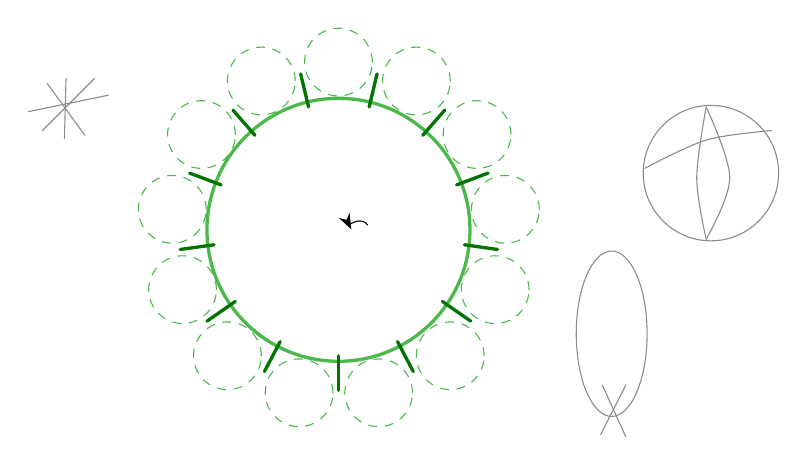
\begin{tikzpicture}[x=1mm,y=1mm,line cap=round,line join=round,font=\scriptsize]
\draw[Lg,very thick] (40.5,-32.4) circle[radius=16.7];
\draw[Lg,dashed] (40.5,-11.1) ellipse[x radius=4.3, y radius=4.3];
\draw[Lg,dashed] (30.7,-13.5) ellipse[x radius=4.3, y radius=4.3];
\draw[Lg,dashed] (23.1,-20.3) ellipse[x radius=4.3, y radius=4.3];
\draw[Lg,dashed] (19.4,-29.8) ellipse[x radius=4.3, y radius=4.3];
\draw[Lg,dashed] (20.7,-40) ellipse[x radius=4.3, y radius=4.3];
\draw[Lg,dashed] (26.4,-48.4) ellipse[x radius=4.3, y radius=4.3];
\draw[Lg,dashed] (35.5,-53.1) ellipse[x radius=4.3, y radius=4.3];
\draw[Lg,dashed] (45.6,-53.1) ellipse[x radius=4.3, y radius=4.3];
\draw[Lg,dashed] (54.7,-48.4) ellipse[x radius=4.3, y radius=4.3];
\draw[Lg,dashed] (60.4,-40) ellipse[x radius=4.3, y radius=4.3];
\draw[Lg,dashed] (61.7,-29.8) ellipse[x radius=4.3, y radius=4.3];
\draw[Lg,dashed] (58.1,-20.3) ellipse[x radius=4.3, y radius=4.3];
\draw[Lg,dashed] (50.4,-13.5) ellipse[x radius=4.3, y radius=4.3];
\draw[Dg,very thick] (36.7,-16.8) -- (35.7,-12.6);
\draw[Dg,very thick] (29.9,-20.4) -- (27.1,-17.2);
\draw[Dg,very thick] (25.6,-26.7) -- (21.6,-25.2);
\draw[Dg,very thick] (24.7,-34.3) -- (20.4,-34.9);
\draw[Dg,very thick] (27.4,-41.5) -- (23.8,-44);
\draw[Dg,very thick] (33.1,-46.6) -- (31.1,-50.4);
\draw[Dg,very thick] (40.5,-48.4) -- (40.5,-52.8);
\draw[Dg,very thick] (48,-46.6) -- (50,-50.4);
\draw[Dg,very thick] (53.7,-41.5) -- (57.3,-44);
\draw[Dg,very thick] (56.5,-34.3) -- (60.7,-34.9);
\draw[Dg,very thick] (55.5,-26.7) -- (59.5,-25.2);
\draw[Dg,very thick] (51.2,-20.4) -- (54,-17.2);
\draw[Dg,very thick] (44.4,-16.8) -- (45.4,-12.6);
\draw[-{Stealth[length=2mm]}] (44.2,-31.8) arc[start angle=20, end angle=200, x radius=1.1, y radius=0.8];
\draw[pencil] (87.8,-25.2) circle[radius=8.6];
\draw[pencil] plot[smooth, tension=0.55] coordinates {(87.2,-16.8) (86,-25.8) (87.2,-33.6)};
\draw[pencil] plot[smooth, tension=0.55] coordinates {(87.2,-16.8) (90.2,-25.8) (87.2,-33.6)};
\draw[pencil] plot[smooth, tension=0.55] coordinates {(79.4,-24.6) (87.2,-21) (95.5,-19.8)};
\draw[pencil] (75.2,-45.6) ellipse[x radius=4.5, y radius=10.5];
\draw[pencil] (74,-52.1) -- (77,-58.7);
\draw[pencil] (77,-52.1) -- (73.8,-58.4);
\draw[pencil] (1.1,-17.4) -- (11.3,-15.3);
\draw[pencil] (3.5,-13.8) -- (8.3,-20.4);
\draw[pencil] (5.9,-13.2) -- (5.7,-20.8);
\draw[pencil] (9.5,-13.2) -- (2.9,-19.8);
\end{tikzpicture}
\end{document}
